% Beamer presentation
\documentclass[11pt,aspectratio=43,ignorenonframetext,t]{beamer}

% Presentation settings
\mode<presentation>{
  \usetheme[framenumber,titleframestart=1]{UoM_alex}
  \usefonttheme{professionalfonts} % using non standard fonts for beamer
  \usefonttheme{serif}
  \usepackage{fontspec}
  \setmainfont[Ligatures=TeX]{Arial}
}

% Handout settings
\mode<article>{
  \usepackage{fullpage}
  \usepackage{fontspec}
  \setmainfont[Ligatures=TeX]{Arial}
  \setlength{\parskip}{1.5\baselineskip} % correct beamer line spacings
  \setlength{\parindent}{0cm}
  \usepackage{enumitem}
  \setlist[itemize]{topsep=0pt}
}

 % Packages
\usepackage{graphicx}
\graphicspath{{./images/png}} % generic graphics path; overridden if necessary
\usepackage{amsmath}
\allowdisplaybreaks[1] % allow eqnarrays to break across pages
\usepackage{amssymb} 
\usepackage[HTML]{xcolor}
\definecolor{uomlinkblue}{HTML}{0071BC}
\usepackage{hyperref}
\hypersetup{
  colorlinks=true,
  linkcolor=uomlinkblue,
  filecolor=uomlinkblue,      
  urlcolor=uomlinkblue,
  pdflang={en-GB},
}
\usepackage[document]{ragged2e} % left aligned text for accessibility
\usepackage{tikz}
\usetikzlibrary{positioning, arrows, arrows.meta}
\usepackage{unicode-math} % unicode maths for accessibility
\usepackage{pdfcomment}   % for alt text for accessibility
\usepackage{rotating}     % allow portrait figures and tables
\usepackage{subfigure}    % allow matrices of figures
\usepackage{float}        % allows H option on floats to force here placement
\usepackage{multirow}     % allows merging of rows in tables
\usepackage{tabularx}     % allows fixed width tables
\usepackage{ctable}       % modifies \hline for use in table
\usepackage{bm}           % allow bold fonts in equations
\usepackage{pgf}          % allow graphics manipulation
\usepackage{etoolbox}
  
% Custom commands
\newcolumntype{Z}{>{\centering\arraybackslash}X}  % tabularx centered columns 

\makeatletter
  \DeclareRobustCommand{\em}
  {
    \@nomath\em
    \if b
      \expandafter\@car\f@series\@nil \normalfont
    \else
      \bfseries
    \fi
  }
\makeatother

\makeatletter
  \preto{\@verbatim}{\topsep=0pt \partopsep=0pt}
\makeatother

\def\checkmark{
  \tikz\fill[scale=0.4](0,.35) -- (.25,0) -- (1,.7) -- (.25,.15) -- cycle;
}

% Counters
\newcounter{example_number} % keep track of the example questions

% Frontmatter
\newcommand{\cmclecture}[1]{
  \title{Combinatorial Mesh Calculus (CMC): Lecture #1}
}
\author{
  Lectured by:
  \href{https://scholar.google.com/citations?user=x4R-snQAAAAJ&hl=en}
  {Dr. Kiprian Berbatov}$^1$\\
  \smallskip
  Lecture Notes Compiled by:
  \href{https://scholar.google.com/citations?user=CoIpITkAAAAJ&hl=en}
  {Muhammad Azeem}$^1$\\
  \smallskip
  Under the supervision of:
  \href{https://scholar.google.co.uk/citations?user=3nWJe5wAAAAJ&hl=en}
  {Prof. Andrey P. Jivkov}$^1$\\
  \smallskip
  {\tiny $^1$Department of Mechanical and Aerospace Engineering,
    The University of Manchester, Oxford Road, Manchester M13 9PL, UK}
}

% Special frames
\newcommand{\cmctitleframe}{
  \titlepage
  \begin{tikzpicture}[remember picture,overlay]
    \node[anchor=south east] at (current page.south east) {
      \href{https://youtube.com/@kipi.berbatov}{
        \includegraphics[width=1.5cm]{youtube-icon.png}
      }
    };
  \end{tikzpicture}
}
\newcommand{\cmcendframe}{
  \begin{figure}
    \centering
    \includegraphics[width=0.85\linewidth]{Thanks.png}
  \end{figure}
}

\cmclecture{12}
\date{31 October 2025}

\begin{document}

%========================= TITLE =========================
\begin{frame}
  \cmctitleframe
\end{frame}


\begin{frame}{Area of a Disk via Green’s Theorem}
\begin{block}{Setup}
For $r>0$, let
\begin{align*}
M=&\overline{B_r}(0,0)=\{(x,y)\in\mathbb{R}^2\mid x^2+y^2\le r^2\},\\
\partial M=&S_r^1=\{(x,y)\in\mathbb{R}^2\mid x^2+y^2=r^2\}.
\end{align*}
The area form on $\mathbb{R}^2$ is $dx\wedge dy$. Since $dx\wedge dy=d(x\,dy)$,
\[
\operatorname{Area}(M)=\int_{M} dx\wedge dy=\int_{M} d(x\,dy)=\int_{\partial M} x\,dy
\quad\text{(Stokes/Green)}.
\]
\end{block}


\end{frame}

\begin{frame}{Parametrization}
\begin{block}{Parametrization and Computation}
Parametrize $\partial M$ by $\gamma(\phi)=(r\cos\phi,r\sin\phi)$, $\phi\in[0,2\pi]$.
Then $x(\phi)=r\cos\phi$, $y(\phi)=r\sin\phi$, so $dy=r\cos\phi\,d\phi$ and
\begin{align*}
\int_{\partial M} x\,dy=&\int_{0}^{2\pi} \bigl(r\cos\phi\bigr)\bigl(r\cos\phi\,d\phi\bigr)\\
=&r^2\int_{0}^{2\pi}\cos^2\phi\,d\phi=r^2\cdot\pi\\=&\pi r^2.
\end{align*}
\end{block}
\end{frame}

\begin{frame}{Visualization}
    \begin{center}
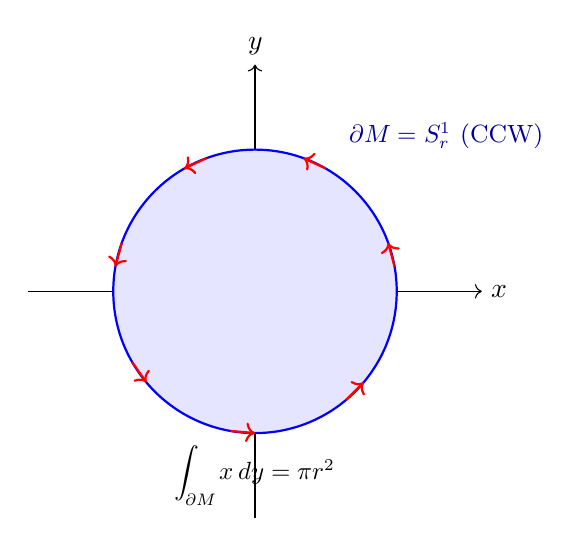
\begin{tikzpicture}[scale=0.9]
% axes
\draw[->] (-3.2,0)--(3.2,0) node[right]{$x$};
\draw[->] (0,-3.2)--(0,3.2) node[above]{$y$};
% disk fill and boundary
\fill[blue!10] (0,0) circle (2);
\draw[thick,blue] (0,0) circle (2);
% orientation arrows on boundary
\foreach \a in {10,60,110,160,210,260,310}{
  \draw[->,red,thick] ({2*cos(\a)},{2*sin(\a)}) -- ({2*cos(\a+10)},{2*sin(\a+10)});
}
\node[blue!60!black] at (2.7,2.2) {\small $\partial M=S_r^1$ (CCW)};
\node at (0,-2.6) {\small $\displaystyle \int_{\partial M} x\,dy=\pi r^2$};
\end{tikzpicture}
\end{center}
\end{frame}

\begin{frame}{Metric Tensor (Riemannian Metric)}
\begin{block}{Definition (Metric)}
Let $M$ be a smooth manifold. A \textbf{metric} on $M$ is a bilinear map
\[
g:\ \mathcal{X}(M)\times\mathcal{X}(M)\longrightarrow\mathcal{F}(M),
\]
satisfying, for all $X,Y\in\mathcal{X}(M)$:
\begin{itemize}
  \item \textit{Symmetry: } $g(X,Y)=g(Y,X)$.
  \item \textit{Positive–definiteness: } $g(X,X)\ge 0$ in $\mathcal{F}(M)$, and $g(X,X)=0$ iff $X=0$.
\end{itemize}
\end{block}

\begin{block}{Riemannian manifold}
Let $M$ be a smooth manifold and $g:\ \mathcal{X}(M)\times\mathcal{X}(M)\longrightarrow\mathcal{F}(M)$ be a metric on $M$. Then the pair $(M,g)$ is a \textbf{Riemannian manifold}.
\end{block}

\end{frame}



\begin{frame}{Metric Examples}
    \begin{block}{Examples in Coordinates}
Fix local coordinates $(x^1,\dots,x^D)$ and frame $\bigl\{\frac{\partial}{\partial x^i}\bigr\}$.
\[
g\!\left(\frac{\partial}{\partial x^i},\frac{\partial}{\partial x^j}\right)=g_{ij}\in\mathcal{F}(M),
\qquad
g=\sum_{i,j=1}^{D} g_{ij}\,dx^i\otimes dx^j,
\]
with the matrix field $\underline{g}=(g_{ij})_{1\le i,j\le D}$ pointwise symmetric positive–definite.
\begin{itemize}
\item \textbf{Euclidean metric on $\mathbb{R}^D$: } $g_{ij}=\delta_{ij}$, i.e.
\[
\underline{g}=I_D=
\begin{pmatrix}
1 & 0 & \cdots & 0\\
0 & 1 & \cdots & 0\\
\vdots & \vdots & \ddots & \vdots\\
0 & 0 & \cdots & 1
\end{pmatrix},
\quad
g=\sum_{i=1}^D dx^i\otimes dx^i.
\]
\end{itemize}
\end{block}
\end{frame}

\begin{frame}{Metric Examples}
\begin{block}{General metric on $\mathbb{R}^D$:}
\begin{itemize}
\item $\underline{g}(x)=(g_{ij}(x))$ with $g_{ij}=g_{ji}$ and
$\underline{g}(x)$ positive–definite for each $x$.
\end{itemize}
\end{block}

\vspace{0.15cm}
\begin{block}{Historical note:}
Bernhard Riemann (1826–1866) introduced Riemannian metrics, founding the intrinsic geometry of manifolds and influencing modern differential geometry and physics.
\end{block}
\end{frame}


\begin{frame}{Musical Isomorphisms}
\begin{block}{Flat, Sharp and Dual Metric}
Given a Riemannian metric $g$, the \textbf{flat} operator
\[
\flat:\ \mathcal{X}(M)\to\Omega^1(M),\qquad (\flat X)(Y)=g(X,Y),
\]
is a $C^\infty(M)$–isomorphism. Its inverse is the \textbf{sharp} operator
\[
\sharp=\flat^{-1}:\ \Omega^1(M)\to\mathcal{X}(M).
\]
They induce a metric on $1$–forms,
\[
g^*:\ \Omega^1(M)\times \Omega^1(M)\to\mathcal{F}(M),\qquad
g^*(\omega,\eta)=\omega(\,\sharp\,\eta\,).
\]
\end{block}
\end{frame}

\begin{frame}{Musical Isomorphisms}
\begin{block}{Flat/Sharp and Dual Metric}
In coordinates, with $g=\sum g_{ij}\,dx^i\otimes dx^j$ and inverse matrix $(g^{ij})$:
\[
g^*=\sum_{i,j=1}^D g^{ij}\,\frac{\partial}{\partial x^i}\otimes \frac{\partial}{\partial x^j}.
\]
\end{block}

\begin{center}
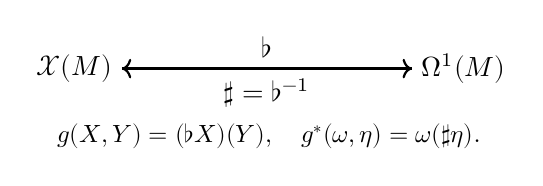
\begin{tikzpicture}[scale=0.95]
% schematic arrows X <-> X^*
\node (XM) at (-2.6,0) {$\mathcal{X}(M)$};
\node (OM) at ( 2.6,0) {$\Omega^1(M)$};
\draw[->,thick] (XM) -- node[above] {$\flat$} (OM);
\draw[->,thick] (OM) -- node[below] {$\sharp=\flat^{-1}$} (XM);
\node at (0,-0.9) {\small $g(X,Y)=(\flat X)(Y),\quad g^*(\omega,\eta)=\omega(\sharp\eta)$.};
\end{tikzpicture}
\end{center}
\end{frame}

\begin{frame}{Pullback Metric on a Submanifold}
\begin{block}{Definition (Induced Metric)}
Let $(M,g)$ be Riemannian and $S\subseteq M$ a smooth submanifold with embedding
$\iota:S\hookrightarrow M$, $\iota(s)=s$.
The \textbf{induced (pullback) metric} on $S$ is
\[
\iota^*g=\sum_{i,j=1}^{D} (g_{ij}\circ \iota)\, d(x^i\circ \iota)\otimes d(x^j\circ \iota).
\]
\end{block}
\begin{block}{Interpretation}
Express $g$ in the ambient coordinates, then pull back each coefficient and
each coordinate differential to $S$ via $\iota$ (i.e.\ \textit{change of variables} to the coordinates on $S$).
\end{block}
\end{frame}

\begin{frame}{Example}
\vspace{-0.2cm}
\begin{block}{Unit Sphere $S^2\subset\mathbb{R}^3$}
Let $M=B_1(0,0,0)=\{(x,y,z)\mid x^2+y^2+z^2\leq1\}$ and $B_1(0,0,0) \subset\mathbb{R}^3$, $S=\partial M=S^2=\{(x,y,z)\mid x^2+y^2+z^2=1\}$ and
$g=dx\otimes dx+dy\otimes dy+dz\otimes dz$ (Euclidean).\\

In spherical coordinates on $S^2$,
\vspace{-0.2cm}
\[
x=\sin\theta\cos\phi,\quad y=\sin\theta\sin\phi,\quad z=\cos\theta,
\]
with
\vspace{-0.2cm}
\[
(\theta,\phi)\in(0,\pi)\times(0,2\pi).
\]
Compute
\vspace{-0.2cm}
\[
\begin{aligned}
dx&=\cos\theta\cos\phi\,d\theta-\sin\theta\sin\phi\,d\phi,\\
dy&=\cos\theta\sin\phi\,d\theta+\sin\theta\cos\phi\,d\phi,\\
dz&=-\sin\theta\,d\theta.
\end{aligned}
\]
\vspace{-0.2cm}
\end{block}
\end{frame}

\begin{frame}{Example}
\vspace{-0.2cm}
\begin{block}{Unit Sphere $S^2\subset\mathbb{R}^3$}
Then
\vspace{-0.2cm}
\[
\iota^*g=dx^2+dy^2+dz^2
=\bigl(d\theta\bigr)^2+\sin^2\theta\,\bigl(d\phi\bigr)^2.
\]
Hence, in the chart $(\theta,\phi)$,
\vspace{-0.2cm}
\[
\underline{h}=
\begin{pmatrix}
1 & 0\\[2pt]
0 & \sin^2\theta
\end{pmatrix},
\qquad
\underline{h}^{-1}=
\begin{pmatrix}
1 & 0\\[2pt]
0 & \dfrac{1}{\sin^2\theta}
\end{pmatrix},
\]
and
\vspace{-0.2cm}
\[
h^{-1}=\frac{\partial}{\partial\theta}\otimes\frac{\partial}{\partial\theta}
+\frac{1}{\sin^2\theta}\,\frac{\partial}{\partial\phi}\otimes\frac{\partial}{\partial\phi}.
\]
\vspace{-0.3cm}
\end{block}
\end{frame}

\begin{frame}{Visualization}
    \begin{center}
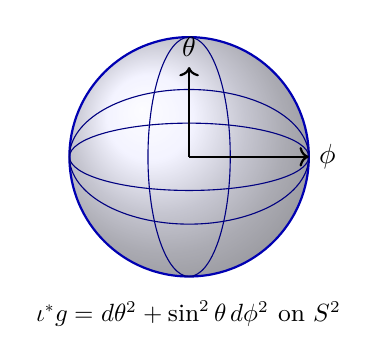
\begin{tikzpicture}[scale=0.95]
% sphere silhouette
\shade[ball color=blue!10,opacity=0.6] (0,0) circle (1.6);
\draw[blue!70!black,thick] (0,0) circle (1.6);
% latitude and longitude (indicative)
\draw[blue!50!black] (0,0) ellipse (1.6 and 0.45);
\draw[blue!50!black] (0,0) ellipse (1.6 and 0.9);
\draw[blue!50!black,rotate=90] (0,0) ellipse (1.6 and 0.55);
% coordinate arrows
\draw[->,thick] (0,0)--(1.6,0) node[right]{$\phi$};
\draw[->,thick] (0,0)--(0,1.2) node[above]{$\theta$};
\node at (0,-2.1) {\small $\iota^*g=d\theta^2+\sin^2\theta\,d\phi^2$ on $S^2$};
\end{tikzpicture}
\end{center}
\end{frame}

\begin{frame}{Orthonormal Frames}
\begin{block}{Definition}
Let $(M,g)$ be a $D$–dimensional Riemannian manifold.
A frame $(X_1,\dots,X_D)$ in $\mathcal{X}(M)$ is \textbf{orthonormal} if
\[
g(X_i,X_j)=\delta_{ij}\qquad(1\le i,j\le D).
\]
The dual coframe (or dual basis) $(\omega^1,\dots,\omega^D)$ in $\Omega^1(M)$ is orthonormal for $g^*$.
\end{block}
\end{frame}

\begin{frame}{Examples of Orthonormal Bases}
\begin{block}{Example 1: Euclidean Space \((\mathbb{R}^D,g=\sum_{i=1}^{D}dx^i\otimes dx^i)\)}
Consider the standard Cartesian coordinates $(x^1,\dots,x^D)$ on $\mathbb{R}^D$.
The standard basis of vector fields is
\[
\left(\frac{\partial}{\partial x^1},\frac{\partial}{\partial x^2},\dots,\frac{\partial}{\partial x^D}\right)
\in\mathcal{X}(\mathbb{R}^D),
\]
and the corresponding dual basis of $1$–forms is
\[
(dx^1,dx^2,\dots,dx^D)\in\Omega^1(\mathbb{R}^D).
\]
For this metric,
\[
g\!\left(\frac{\partial}{\partial x^i},\frac{\partial}{\partial x^j}\right)
=\delta_{ij},\qquad
g^*(dx^i,dx^j)=\delta_{ij}.
\]
\end{block}
\end{frame}


\begin{frame}{Examples of Orthonormal Bases}
\begin{block}{Example 1: Euclidean Space \((\mathbb{R}^D,g=\sum_{i=1}^{D}dx^i\otimes dx^i)\)}
Hence both sets are orthonormal:
\[
g\left(\frac{\partial}{\partial x^i},\frac{\partial}{\partial x^i}\right)=1,
\quad
g\left(\frac{\partial}{\partial x^i},\frac{\partial}{\partial x^j}\right)=0\ (i\ne j),
\]
and similarly for the dual coframe.
\end{block}

\begin{block}{Interpretation:}
The Euclidean metric measures inner products as the usual dot product; hence, in these coordinates, vectors and covectors have the same orthonormal structure.
\end{block}
\end{frame}


\begin{frame}{Visualization}
    \begin{center}
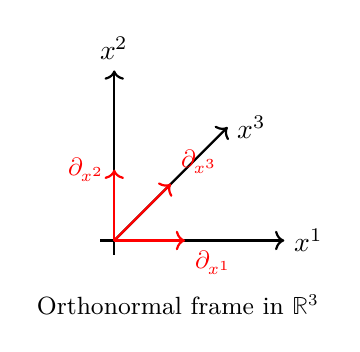
\begin{tikzpicture}[scale=0.9]
% axes
\draw[->,thick] (-0.2,0)--(2.4,0) node[right]{$x^1$};
\draw[->,thick] (0,-0.2)--(0,2.4) node[above]{$x^2$};
\draw[->,thick] (0,0)--(1.6,1.6) node[right]{$x^3$};
% vectors
\draw[->,red,thick] (0,0)--(1,0) node[below right]{\small $\partial_{x^1}$};
\draw[->,red,thick] (0,0)--(0,1) node[left]{\small $\partial_{x^2}$};
\draw[->,red,thick] (0,0)--(0.8,0.8) node[above right]{\small $\partial_{x^3}$};
\node at (0.9,-0.9) {\small Orthonormal frame in $\mathbb{R}^3$};
\end{tikzpicture}
\end{center}
\end{frame}

\begin{frame}{Example 2: Orthonormal Basis}
\vspace{-0.2cm}
\begin{block}{On the Sphere \(S^2\)}
On $S^2$ with the induced metric from $\mathbb{R}^3$,
\vspace{-0.2cm}
\[
h=d\theta^2+\sin^2\theta\,d\phi^2,
\]
where $(\theta,\phi)$ are the standard spherical coordinates:
\vspace{-0.2cm}
\[
x=\sin\theta\cos\phi,\qquad
y=\sin\theta\sin\phi,\qquad
z=\cos\theta.
\]

Compute $h$ on the coordinate vector fields:
\vspace{-0.2cm}
\[
\begin{aligned}
h\!\left(\frac{\partial}{\partial\theta},\frac{\partial}{\partial\theta}\right)
&=1,\\[2pt]
h\!\left(\frac{\partial}{\partial\phi},\frac{\partial}{\partial\phi}\right)
&=\sin^2\theta,
\end{aligned}
\]
\end{block}
\end{frame}

\begin{frame}{Example 2: Orthonormal Basis}
\begin{block}{On the Sphere \(S^2\)}
\[
\begin{aligned}
h\!\left(\frac{\partial}{\partial\theta},\frac{\partial}{\partial\phi}\right)
&=0.
\end{aligned}
\]
Hence, the rescaled frame
\[
\left(\frac{\partial}{\partial\theta},\ \frac{1}{\sin\theta}\frac{\partial}{\partial\phi}\right)
\]
is orthonormal:
\[
h\!\left(\frac{\partial}{\partial\theta},\frac{\partial}{\partial\theta}\right)
=h\!\left(\frac{1}{\sin\theta}\frac{\partial}{\partial\phi},\frac{1}{\sin\theta}\frac{\partial}{\partial\phi}\right)=1,
\quad
h\!\left(\frac{\partial}{\partial\theta},\frac{1}{\sin\theta}\frac{\partial}{\partial\phi}\right)=0.
\]
The dual orthonormal coframe is $(d\theta,\ \sin\theta\,d\phi)$.
\end{block}

\end{frame}

\begin{frame}{Example 2: Orthonormal Basis}
\begin{center}
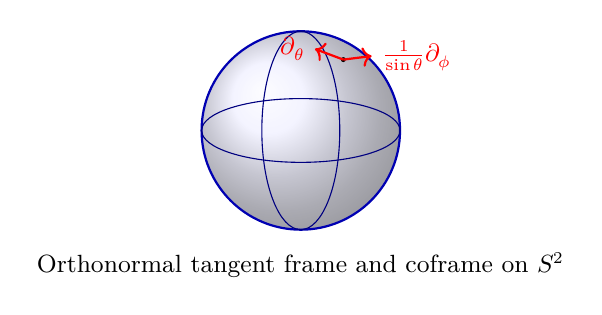
\begin{tikzpicture}[scale=0.9]
% sphere
\shade[ball color=blue!10,opacity=0.6] (0,0) circle (1.4);
\draw[blue!70!black,thick] (0,0) circle (1.4);
% latitude and longitude
\draw[blue!50!black] (0,0) ellipse (1.4 and 0.45);
\draw[blue!50!black,rotate=90] (0,0) ellipse (1.4 and 0.55);
% tangent point
\fill (0.6,1.0) circle (1pt);
\draw[->,red,thick] (0.6,1.0)--(0.2,1.15) node[left]{\small $\partial_\theta$};
\draw[->,red,thick] (0.6,1.0)--(1.0,1.05) node[right]{\small $\frac{1}{\sin\theta}\partial_\phi$};
\node at (0,-1.9) {\small Orthonormal tangent frame and coframe on $S^2$};
\end{tikzpicture}
\end{center}
\end{frame}




\begin{frame}{Inner Product on Differential Forms}
\begin{block}{Definition}
Let $(M,g)$ be a $D$–dimensional Riemannian manifold.
The metric $g$ induces an inner product on $p$–forms:
\[
g^*_p:\ \Omega^p(M)\times \Omega^p(M)\to \mathcal{F}(M),
\qquad p=0,1,\dots,D,
\]
defined recursively:
\[
\begin{aligned}
g^*_0(f_1,f_2) &= f_1 f_2, & f_1,f_2\in\mathcal{F}(M),\\
g^*_1(\omega,\eta) &= g^*(\omega,\eta), & \omega,\eta\in\Omega^1(M),\\[2pt]
\end{aligned}
\]
\end{block}
\end{frame}

\begin{frame}{Inner Product on $p$–Forms}
\begin{block}{Definition}
Let $(M,g)$ be a $D$–dimensional Riemannian manifold.
For $p\ge2$, the metric $g$ induces an inner product on $p$–forms
\[
g^*_p:\Omega^p(M)\times\Omega^p(M)\longrightarrow\mathcal{F}(M),
\]
defined on decomposable forms as
\[
g^*_p(\omega_1\wedge\dots\wedge\omega_p,\,
\eta_1\wedge\dots\wedge\eta_p)
=
\begin{vmatrix}
g^*(\omega_1,\eta_1) & g^*(\omega_1,\eta_2) & \cdots & g^*(\omega_1,\eta_p)\\[4pt]
g^*(\omega_2,\eta_1) & g^*(\omega_2,\eta_2) & \cdots & g^*(\omega_2,\eta_p)\\[4pt]
\vdots & \vdots & \ddots & \vdots\\[4pt]
g^*(\omega_p,\eta_1) & g^*(\omega_p,\eta_2) & \cdots & g^*(\omega_p,\eta_p)
\end{vmatrix}.
\]
\end{block}
\end{frame}

\begin{frame}{Explanation}
\begin{block}{}
The determinant encodes all mutual inner products between $\{\omega_i\}$ and $\{\eta_j\}$:
\[
g^*_p(\omega_1\!\wedge\!\dots\!\wedge\!\omega_p,\eta_1\!\wedge\!\dots\!\wedge\!\eta_p)
=\!\!\sum_{\sigma\in S_p}\!\!\mathrm{sgn}(\sigma)
\prod_{k=1}^{p} g^*(\omega_k,\eta_{\sigma(k)}),
\]
where $S_p$ is the permutation group on $\{1,\dots,p\}$ and $\mathrm{sgn}(\sigma)$ is the sign of permutation $\sigma$.
This generalizes the usual Euclidean determinant form of the inner product on wedge products.
\end{block}

\begin{center}
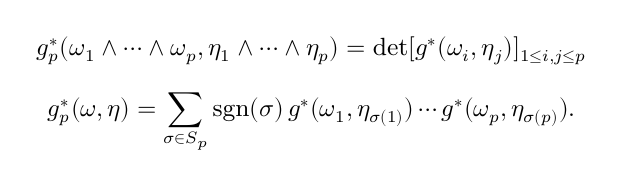
\begin{tikzpicture}[scale=0.9]
\node at (0,0) {\small $g^*_p(\omega_1\wedge\dots\wedge\omega_p,\eta_1\wedge\dots\wedge\eta_p)
=\det[g^*(\omega_i,\eta_j)]_{1\le i,j\le p}$};
\node at (0,-1.0) {\small $\displaystyle g^*_p(\omega,\eta)
=\sum_{\sigma\in S_p}\mathrm{sgn}(\sigma)
\,g^*(\omega_1,\eta_{\sigma(1)})\cdots g^*(\omega_p,\eta_{\sigma(p)}).$};
\end{tikzpicture}
\end{center}
\end{frame}


\begin{frame}{Example}
\vspace{-0.3cm}
\begin{block}{$S^2$ with $h=d\theta^2+\sin^2\theta\,d\phi^2$}
\vspace{-0.8cm}
\begin{align*}
g_2^*(d\theta\wedge d\phi,\ d\theta\wedge d\phi)
=&\det
\begin{pmatrix}
g^*(d\theta,d\theta) & g^*(d\theta,d\phi)\\
g^*(d\phi,d\theta) & g^*(d\phi,d\phi)
\end{pmatrix}\\
=&\det
\begin{pmatrix}
1 & 0\\
0 & \dfrac{1}{\sin^2\theta}
\end{pmatrix}
=\dfrac{1}{\sin^2\theta}.
\end{align*}
Hence
\vspace{-0.7cm}
\[
g_2^*(\sin\theta\,d\theta\wedge d\phi,\ \sin\theta\,d\theta\wedge d\phi)
=\sin^2\theta\cdot\dfrac{1}{\sin^2\theta}=1.
\]
\end{block}
\vspace{-0.9cm}
\begin{center}
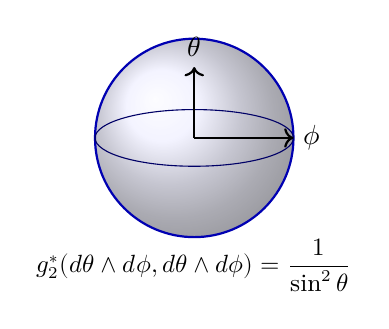
\begin{tikzpicture}[scale=0.9]
\shade[ball color=blue!10,opacity=0.6] (0,0) circle (1.4);
\draw[blue!70!black,thick] (0,0) circle (1.4);
\draw[blue!40!black] (0,0) ellipse (1.4 and 0.4);
\draw[->,thick] (0,0)--(1.4,0) node[right]{$\phi$};
\draw[->,thick] (0,0)--(0,1.0) node[above]{$\theta$};
\node at (0,-1.8) {\small $g_2^*(d\theta\wedge d\phi,d\theta\wedge d\phi)=\dfrac{1}{\sin^2\theta}$};
\end{tikzpicture}
\end{center}
\end{frame}

\begin{frame}{Volume Form}
\begin{block}{Definition}
Let $(M,g)$ be a $D$–dimensional Riemannian manifold.
Since $\Omega^D(M)$ is $1$–dimensional,
there exist (up to sign) two $D$–forms $\omega$ and $-\omega$
such that
\[
g^*_D(\omega,\omega)=1.
\]
Any such form is a \textbf{volume form} of $(M,g)$.
If $M$ is oriented, the sign of $\omega$ is fixed canonically,
and we denote $\mathrm{vol}_g=\omega$.
\end{block}
\end{frame}

\begin{frame}{Examples}
    \begin{block}{Example}
\begin{itemize}
\item On $\mathbb{R}^D$ with $g=\sum dx^i\otimes dx^i$:
\[
\mathrm{vol}_g=\pm\,dx^1\wedge dx^2\wedge\dots\wedge dx^D.
\]
\item On $S^2$ with $h=d\theta^2+\sin^2\theta\,d\phi^2$:
\[
\mathrm{vol}_h=\sin\theta\,d\theta\wedge d\phi.
\]
\end{itemize}
\end{block}
\end{frame}

\begin{frame}{Proposition}
\begin{block}{Statement: Volume Form from Orthonormal Basis}
Let $(M,g)$ be an oriented $D$–dimensional Riemannian manifold and
$e^1,\dots,e^D$ an orthonormal basis of $\Omega^1(M)$ consistent with the orientation.
Then
\[
\mathrm{vol}_g=e^1\wedge e^2\wedge\dots\wedge e^D.
\]
\end{block}
\end{frame}

\begin{frame}{Examples}
\vspace{-0.2cm}
    \begin{block}{Example}
\begin{itemize}
\item On $(\mathbb{R}^D,g)$ with standard basis $dx^1,\dots,dx^D$:
\vspace{-0.2cm}
\[
\mathrm{vol}_g=dx^1\wedge dx^2\wedge\dots\wedge dx^D.
\]
\item On $S^2$ with orthonormal coframe $(d\theta,\sin\theta\,d\phi)$:
\vspace{-0.2cm}
\[
\mathrm{vol}_h=d\theta\wedge(\sin\theta\,d\phi)=\sin\theta\,d\theta\wedge d\phi.
\]
\end{itemize}
\end{block}
\vspace{-0.2cm}
\begin{center}
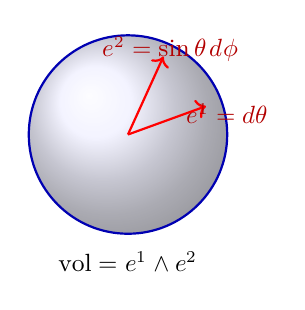
\begin{tikzpicture}[scale=0.9]
\shade[ball color=blue!10,opacity=0.6] (0,0) circle (1.4);
\draw[blue!70!black,thick] (0,0) circle (1.4);
\draw[->,thick,red] (0,0)--(1.1,0.4);
\draw[->,thick,red] (0,0)--(0.5,1.1);
\node[red!70!black] at (1.4,0.3) {\small $e^1=d\theta$};
\node[red!70!black] at (0.6,1.2) {\small $e^2=\sin\theta\,d\phi$};
\node at (0,-1.8) {\small $\mathrm{vol}=e^1\wedge e^2$};
\end{tikzpicture}
\end{center}
\end{frame}

\begin{frame}{Hodge Star Operator}
\begin{block}{Definition}
Let $(M,g)$ be a $D$–dimensional oriented Riemannian manifold with volume form $\mathrm{vol}_g$.
The \textbf{Hodge star} is the unique $\mathcal{F}(M)$–linear map
\[
\star_p:\Omega^p(M)\to \Omega^{D-p}(M)
\]
such that for all $\omega,\eta\in\Omega^p(M)$,
\[
g^*_p(\omega,\eta)\,\mathrm{vol}_g=\omega\wedge\star_p\eta.
\]
Equivalently, for $\omega\in\Omega^p(M)$, $\eta\in\Omega^{D-p}(M)$,
\[
g^*_{D-p}(\star_p\omega,\eta)\,\mathrm{vol}_g=\omega\wedge\eta.
\]
\end{block}
\end{frame}

% ----------------------------------------------------------
\begin{frame}{Theorem: Properties of the Hodge Star}
\begin{block}{Statement}
Let $(M,g)$ be an oriented $D$–dimensional Riemannian manifold and
$e^1,\dots,e^D$ be an oriented orthonormal basis of $\Omega^1(M)$.
\begin{enumerate}
\item For an index set $I=\{i_1<\dots<i_p\}$,
let $e^I=e^{i_1}\wedge\dots\wedge e^{i_p}$,
and $J$ the complementary set of indices.
Then
\[
\star_p e^I=s\,e^J,\quad s\in\{-1,1\},
\]
where $e^I\wedge e^J=s\,\mathrm{vol}_g=s\,e^1\wedge\dots\wedge e^D$.
\item $\displaystyle \star_{D-p}\circ\star_p=(-1)^{p(D-p)}\,\mathrm{id}_{\Omega^p(M)}$.\\

In particular, if $D$ is odd, $\star_{D-p}\circ\star_p=\mathrm{id}_{\Omega^p(M)}$.
\end{enumerate}
\end{block}
\end{frame}

% ----------------------------------------------------------
\begin{frame}{Examples: Hodge Star in $D=2$}
\begin{block}{Example: $S^2$ with orthonormal coframe $(e^1=d\theta,\ e^2=\sin\theta\,d\phi)$}
\[
\begin{aligned}
&\star_0(1)=e^1\wedge e^2=\mathrm{vol},\\
&\star_1(e^1)=e^2,\qquad \star_1(e^2)=-e^1,\\
&\star_2(\mathrm{vol})=\star_2(e^1\wedge e^2)=1.
\end{aligned}
\]
\end{block}

\begin{center}
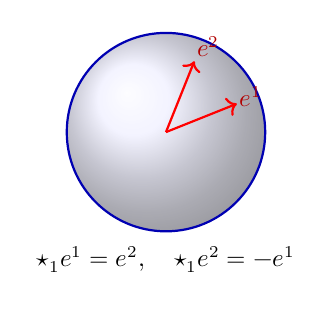
\begin{tikzpicture}[scale=0.9]
\shade[ball color=blue!10,opacity=0.6] (0,0) circle (1.4);
\draw[blue!70!black,thick] (0,0) circle (1.4);
\draw[->,thick,red] (0,0)--(1.0,0.4);
\draw[->,thick,red] (0,0)--(0.4,1.0);
\node[red!70!black] at (1.2,0.5) {\small $e^1$};
\node[red!70!black] at (0.6,1.2) {\small $e^2$};
\node at (0,-1.8) {\small $\star_1 e^1=e^2,\quad \star_1 e^2=-e^1$};
\end{tikzpicture}
\end{center}
\end{frame}

% ----------------------------------------------------------
\begin{frame}{Examples: Hodge Star in $D=3$}
\begin{block}{Example: $\mathbb{R}^3$ with orthonormal coframe $(e^1=dx,\ e^2=dy,\ e^3=dz)$}
\[
\begin{aligned}
&\star_0(1)=e^1\wedge e^2\wedge e^3=\mathrm{vol},\\
&\star_1(e^1)=e^2\wedge e^3,\quad \star_1(e^2)=e^3\wedge e^1,\quad \star_1(e^3)=e^1\wedge e^2,\\
&\star_2(e^1\wedge e^2)=e^3,\quad \star_2(e^2\wedge e^3)=e^1,\quad \star_2(e^3\wedge e^1)=e^2,\\
&\star_3(e^1\wedge e^2\wedge e^3)=1.
\end{aligned}
\]
\end{block}

\begin{center}
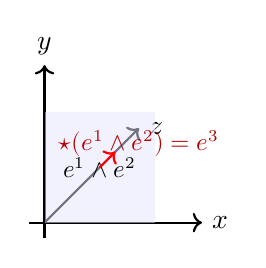
\begin{tikzpicture}[scale=1.0]
% coordinate axes cube
\draw[->,thick] (-0.2,0)--(2.0,0) node[right]{$x$};
\draw[->,thick] (0,-0.2)--(0,2.0) node[above]{$y$};
\draw[->,thick] (0,0)--(1.2,1.2) node[right]{$z$};
% plane patches
\fill[blue!10,opacity=0.5] (0,0)--(1.4,0)--(1.4,1.4)--(0,1.4)--cycle;
\node at (0.7, 0.7) {\small $e^1\wedge e^2$};
\draw[->,red,thick] (0.7,0.7)--(0.9,0.9);
\node[red!70!black] at (1.2,1.0) {\small $\star(e^1\wedge e^2)=e^3$};
\end{tikzpicture}
\end{center}
\end{frame}





% ----------------------------------------------------------
\begin{frame}{Summary}
\begin{block}{}
\begin{itemize}
\item Area of a disk via Green/Stokes: $\displaystyle \operatorname{Area}(\overline{B_r})=\int_{\partial B_r} x\,dy=\pi r^2$.
\item Riemannian metric $g$ gives lengths/angles: $g=\sum g_{ij}\,dx^i\otimes dx^j$, with inverse $g^*=\sum g^{ij}\,\partial_i\otimes\partial_j$.
\item Musical isomorphisms $\flat,\sharp$ identify vectors and $1$–forms.
\item Induced metric on submanifolds: $\iota^*g$; for $S^2$, $d\theta^2+\sin^2\theta\,d\phi^2$.
\item Orthonormal frames simplify computations (e.g.\ on $S^2$: $(\partial_\theta,\frac{1}{\sin\theta}\partial_\phi)$).
\item $g^*_p$ defines inner products on all $p$–forms via determinant of $g^*(\cdot,\cdot)$.
\end{itemize}
\end{block}
\end{frame}

\begin{frame}{Summary}
\begin{block}{}
\begin{itemize}
\item Volume form $\mathrm{vol}_g$ satisfies $g^*_D(\mathrm{vol}_g,\mathrm{vol}_g)=1$ and encodes orientation.
\item $\mathrm{vol}_g=e^1\wedge\dots\wedge e^D$ for any oriented orthonormal coframe.
\item Hodge star $\star_p$ maps $\Omega^p(M)\to\Omega^{D-p}(M)$ satisfying
$g^*_p(\omega,\eta)\mathrm{vol}_g=\omega\wedge\star_p\eta$.
\item Key identity: $\star_{D-p}\circ\star_p=(-1)^{p(D-p)}\mathrm{id}$.
\end{itemize}
\end{block}
\end{frame}


\begin{frame}{Thanks}
  \cmcendframe
\end{frame}

\end{document}
